\chapter{Electrons in Solids}\label{ch:b3:electrons-in-solids}

% Provenance (not for print): second half of the "physique du solide"
% module (Drude, Sommerfeld, bands, semiconductors) common to the
% surveyed third-year curricula.

Copper conducts electricity a million billion billion times better
than quartz --- the widest range of any physical property, commanded
by materials that look like grey lumps either way. The scaffolding of
the last chapter explains none of it; the \emph{electrons} poured into
it explain all of it. This chapter runs the century's three passes at
the problem, each inheriting the last's wreckage: Drude's classical
pinball (1900), which gets Ohm's law right and the heat capacity
scandalously wrong; Sommerfeld's Fermi gas, which is
\cref{ch:b3:quantum-statistics} cashing its cheque; and Bloch's
insight that an electron wave in a periodic \omterm{def:b3:crystalline-solids:lattice}{lattice} Bragg-reflects
like any other wave --- opening \emph{\omterm{thm:b3:electrons-in-solids:bloch}{band gaps}} that sort all solids
into \omterm{def:b3:electrons-in-solids:classes}{metals}, \omterm{def:b3:electrons-in-solids:classes}{insulators}, and the narrow-gap middle children,
\omterm{def:b3:electrons-in-solids:classes}{semiconductors}, on which the whole electronic age is built. The
chapter ends inside a solar panel.

\section{Drude's pinball metal}

\begin{proposition}[The Drude conductivity]\label{prop:b3:electrons-in-solids:drude}
\index{Drude model}\index{conductivity!microscopic}\index{drift velocity}
Treat a \omterm{def:b3:electrons-in-solids:classes}{metal}'s valence electrons as a classical gas, density $n$,
bouncing off obstacles every $\tau$ seconds. A field $\vect E$
accelerates each between collisions; the average \emph{\omterm{prop:b3:electrons-in-solids:drude}{drift
velocity}} is $\vect v_{\text{d}} = -e\tau\vect E/m_{\text{e}}$,
tiny beside the thermal motion. The current density $\vect j =
-ne\vect v_{\text{d}}$ then obeys Ohm's law locally,
$\vect j = \sigma\vect E$, with
\[
\sigma = \frac{ne^2\tau}{m_{\text{e}}} .
\]
Copper's measured $\sigma$ demands $\tau \approx \qty{2.5e-14}{s}$
--- and the model's two glories follow: it explains why resistors
heat (the field's work is thermalised each collision), and it
predicts the Wiedemann--Franz law, that $\kappa/\sigma T$ is the
same constant for all \omterm{def:b3:electrons-in-solids:classes}{metals} --- electrons carry both charge and
heat (\cref{exo:b3:electrons-in-solids:5}).
\end{proposition}

\begin{proof}
Between collisions $\dot{\vect v} = -e\vect E/m_{\text{e}}$;
starting afresh at each collision, the mean velocity acquired in a
mean time $\tau$ is $-e\tau\vect E/m_{\text{e}}$. Then $\vect j =
-ne\vect v_{\text{d}} = (ne^2\tau/m_{\text{e}})\vect E$.
\end{proof}

\begin{omfigure}
\begin{tikzpicture}[scale=1.0]
  % ion grid
  \foreach \x in {0,1.3,...,7.9}
    \foreach \y in {0,1.1,2.2}
      \draw[omDef!50, fill=omDef!12] (\x,\y) circle (5.5pt);
  % zigzag electron path with slight downfield drift
  \draw[omThm, thick, ->]
    (0.25,1.62) -- (1.0,0.55) -- (1.9,1.7) -- (2.6,0.6) -- (3.6,1.55)
    -- (4.3,0.45) -- (5.25,1.6) -- (5.95,0.5) -- (6.9,1.5) -- (7.65,0.7);
  % field and drift arrows
  \draw[->, thick] (2.6,3.0) -- (1.2,3.0)
    node[midway, above, font=\scriptsize] {$\vect E$};
  \draw[->, thick, omThm, dashed] (5.0,3.0) -- (6.8,3.0)
    node[midway, above, font=\scriptsize]
    {drift $\vect v_{\text{d}}$};
\end{tikzpicture}

{\small Drude's picture: an electron ricochets at
$\sim\qty{e6}{m/s}$, while the field superimposes a drift of
fractions of a millimetre per second
(\cref{exo:b3:electrons-in-solids:2}). Ohm's law drops out; the
model's failures taught more still.}
\end{omfigure}

\begin{remark}[Sommerfeld's rescue]\label{rem:b3:electrons-in-solids:sommerfeld}
\index{Sommerfeld model}\index{Fermi energy!in metals}
Drude's gas should add $\tfrac32k_{\text{B}}$ per electron to a
\omterm{def:b3:electrons-in-solids:classes}{metal}'s heat capacity; experiment finds a hundred times less.
\Cref{ch:b3:quantum-statistics} already acquitted the electrons:
they are a \emph{degenerate Fermi gas}, $T_{\text{F}} \sim
\qty{8e4}{K}$, and only the thermal shell within
$k_{\text{B}}T$ of the Fermi surface can respond --- to heat, and
to scattering. Sommerfeld's re-run of Drude with Fermi--Dirac
statistics keeps the conductivity formula (with $\tau$ now the
lifetime of Fermi-surface electrons, whose \qty{e6}{m/s} is
$v_{\text{F}}$, not thermal speed), fixes the heat capacity to its
measured $T/T_{\text{F}}$ sliver, and even repairs
Wiedemann--Franz's numerical constant. One mystery survives every
free-electron model: why quartz will not conduct at all.
\end{remark}

\section{Bloch: the lattice speaks}

\begin{theorem}[Bloch states and band gaps]\label{thm:b3:electrons-in-solids:bloch}
\index{Bloch's theorem}\index{band gap}\index{band structure}
In a perfect periodic potential, the stationary states are
\emph{Bloch waves} $\psi_k(x) = u_k(x)\eu^{\iu kx}$ ---
plane waves dressed with the \omterm{def:b3:crystalline-solids:lattice}{lattice}'s own periodicity $u_k$ ---
which propagate \emph{without scattering}: a perfect \omterm{def:b3:crystalline-solids:lattice}{crystal} has
zero resistance, and real resistance comes from imperfections
(vibrations, impurities). But not all energies survive. At
$k = \pi/a$ the electron's wavelength is $2a$: Bragg's condition
on the \omterm{def:b3:crystalline-solids:lattice}{lattice} itself (\cref{thm:b3:crystalline-solids:dispersion}
made the same discovery for sound). The reflected and incident
waves form two standing patterns --- charge piled on the ions
(lower energy) or between them (higher) --- so the free-electron
parabola $E = \hbar^2k^2/2m_{\text{e}}$ tears open: an interval of
forbidden energies, the \emph{\omterm{thm:b3:electrons-in-solids:bloch}{band gap}} $E_{\text{g}}$, separates
a filled-out \emph{band} of allowed states from the next. A
\omterm{def:b3:crystalline-solids:lattice}{crystal}'s electronic identity is its ladder of bands and gaps.
\end{theorem}
\admitted

\begin{omfigure}
\begin{tikzpicture}
  \begin{axis}[omaxis, axis x line=bottom, axis y line=left,
    width=9.6cm, height=6.2cm, xmin=0, xmax=5.4, ymin=0, ymax=2.6,
    xlabel={$k$}, ylabel={$E$},
    xlabel style={at={(axis description cs:0.5,-0.1)}, anchor=north},
    xtick={3.1416}, xticklabels={$\pi/a$}, ytick=\empty, clip=true]
    % free-electron parabola (dashed)
    \addplot[gray, dashed, domain=0:5.1, samples=120] {x*x/10};
    % lower band: bends flat at zone edge
    \addplot[omDef, very thick, domain=0:3.1416, samples=120]
      {x*x/10 - 0.18*(x/3.1416)^6};
    % upper band
    \addplot[omDef, very thick, domain=3.1416:5.1, samples=120]
      {x*x/10 + 0.18*((5.1-x)/1.9584)^2};
    \draw[gray, dashed] (axis cs:3.1416,0) -- (axis cs:3.1416,2.55);
    % gap markers
    \draw[omThm, thick, <->] (axis cs:3.2,0.81) -- (axis cs:3.2,1.16);
    \node[omThm, font=\scriptsize, anchor=west] at (axis cs:3.34,0.98)
      {gap $E_{\text{g}}$};
    \node[gray, font=\scriptsize, anchor=north west, align=left]
      at (axis cs:0.35,2.45) {dashed: free electron};
    \node[omDef, font=\scriptsize, anchor=east] at (axis cs:2.75,0.35)
      {band 1};
    \node[omDef, font=\scriptsize, anchor=west] at (axis cs:3.6,2.35)
      {band 2};
  \end{axis}
\end{tikzpicture}

{\small The nearly-free electron. Away from the zone edge the
electron barely notices the \omterm{def:b3:crystalline-solids:lattice}{lattice}; at $k = \pi/a$ its own Bragg
reflection splits the parabola, forbidding the energies in the
gap. Sound waves did exactly this in the last chapter --- same
\omterm{def:b3:crystalline-solids:lattice}{lattice}, same interference, new tenant.}
\end{omfigure}

\begin{definition}[Metals, insulators, semiconductors]\label{def:b3:electrons-in-solids:classes}
\index{metal}\index{insulator}\index{semiconductor}
Fill the bands with the \omterm{def:b3:crystalline-solids:lattice}{crystal}'s electrons, two per state
(\cref{ch:b3:identical-particles}), coldest first. If the topmost
occupied band is \emph{partly} filled, infinitesimal energy can
shift electrons into net motion: a \emph{metal} (sodium: one
valence electron, half a band; divalent metals conduct through
overlapping bands). If it is \emph{exactly} full, with a wide gap
above, no small push can rearrange anything: an \emph{insulator}
(diamond, $E_{\text{g}} = \qty{5.5}{eV}$). If the gap is small ---
$\qty{1.12}{eV}$ in silicon --- thermal agitation hoists a few
electrons across, each leaving a mobile \emph{\omterm{def:b3:electrons-in-solids:doping}{hole}} below: a
\emph{semiconductor}, whose carrier count
$\propto\eu^{-E_{\text{g}}/2k_{\text{B}}T}$ doubles every few
degrees. Hence the great divide: metals conduct worse when heated
(more vibrations to scatter off), semiconductors better
(exponentially more carriers) --- one sign flip that identifies a
material's class in a single measurement.
\end{definition}

\begin{omfigure}
\begin{tikzpicture}[scale=1.0]
  % metal: half-filled band
  \begin{scope}
    \fill[omDef!25] (0,0) rectangle (1.8,0.8);
    \draw[thick] (0,0) rectangle (1.8,1.6);
    \node[font=\scriptsize, anchor=north] at (0.9,-0.15) {metal};
    \node[font=\tiny, anchor=south] at (0.9,1.65) {partly filled};
  \end{scope}
  % insulator
  \begin{scope}[xshift=3.6cm]
    \fill[omDef!25] (0,0) rectangle (1.8,0.9);
    \draw[thick] (0,0) rectangle (1.8,0.9);
    \draw[thick] (0,2.1) rectangle (1.8,2.9);
    \draw[omThm, thick, <->] (2.05,0.9) -- (2.05,2.1);
    \node[omThm, font=\tiny, anchor=west] at (2.12,1.5)
      {$E_{\text{g}} \sim \qty{5}{eV}$};
    \node[font=\scriptsize, anchor=north] at (0.9,-0.15) {insulator};
    \node[font=\tiny, anchor=south] at (0.9,2.95) {empty};
  \end{scope}
  % semiconductor
  \begin{scope}[xshift=8.4cm]
    \fill[omDef!25] (0,0) rectangle (1.8,0.9);
    \draw[thick] (0,0) rectangle (1.8,0.9);
    \draw[thick] (0,1.5) rectangle (1.8,2.3);
    \draw[omThm, thick, <->] (2.05,0.9) -- (2.05,1.5);
    \node[omThm, font=\tiny, anchor=west] at (2.12,1.2)
      {$\sim\qty{1}{eV}$};
    % thermally excited carriers
    \fill[omThm] (0.5,1.62) circle (1.6pt);
    \fill[omThm] (1.25,1.62) circle (1.6pt);
    \draw[omThm] (0.5,0.78) circle (1.6pt);
    \draw[omThm] (1.25,0.78) circle (1.6pt);
    \node[font=\scriptsize, anchor=north] at (0.9,-0.15) {semiconductor};
    \node[font=\tiny, anchor=south] at (0.9,2.35)
      {a few electrons $+$ holes};
  \end{scope}
\end{tikzpicture}

{\small Band filling decides everything. A partly filled band
conducts; a full band under a wide gap cannot; a narrow gap lets
temperature (or light, or \omterm{def:b3:electrons-in-solids:doping}{doping}) negotiate --- the \omterm{def:b3:electrons-in-solids:classes}{semiconductor}'s
entire usefulness is that its conductivity is \emph{adjustable}.}
\end{omfigure}

\section{Engineering the gap: doping and the junction}

\begin{definition}[Doping]\label{def:b3:electrons-in-solids:doping}
\index{doping}\index{donor}\index{acceptor}\index{hole}
Replace one silicon atom in a million by phosphorus (five valence
electrons): four bonds are satisfied and the fifth electron,
bound by a mere \qty{45}{meV}
(\cref{exo:b3:electrons-in-solids:10}), is free at room
temperature. Such \emph{donors} make an \emph{n-type}
\omterm{def:b3:electrons-in-solids:classes}{semiconductor}, conduction by electrons; boron (three electrons)
is an \emph{acceptor}, grabbing a bond electron and releasing a
mobile \emph{hole} --- a missing electron that moves, responds to
fields, and carries positive charge as genuinely as a bubble
carries buoyancy: \emph{p-type}. Doping swings the carrier density
--- and hence conductivity --- across six orders of magnitude at
will: the knob that turns sand into circuitry.
\end{definition}

\begin{proposition}[The p--n junction]\label{prop:b3:electrons-in-solids:junction}
\index{p--n junction}\index{diode}\index{depletion zone}
Join p-type to n-type. Electrons spill toward the \omterm{def:b3:electrons-in-solids:doping}{holes} and
annihilate them near the interface, exposing a \emph{\omterm{prop:b3:electrons-in-solids:junction}{depletion
zone}} of fixed ionised dopants whose double layer builds an
internal field --- equilibrium at the built-in voltage
$V_{\text{bi}} = (k_{\text{B}}T/e)
\ln(N_{\text{a}}N_{\text{d}}/n_{\text{i}}^2) \approx
\qty{0.7}{V}$ in silicon. The junction then rectifies: forward
bias lowers the barrier and current grows as
$\eu^{eV/k_{\text{B}}T}$; reverse bias raises it and only a
leakage $I_0$ flows:
\[
I = I_0\big(\eu^{eV/k_{\text{B}}T} - 1\big) .
\]
This asymmetry is the \emph{diode} --- and, run in its variants,
the LED (recombining pairs emit gap-energy photons), the solar
cell (gap-energy photons create pairs that the built-in field
sweeps out: \cref{pb:b3:electrons-in-solids:1}), and, doubled
into sandwiches, the transistor: the switch of which a modern
chip prints hundreds of billions.
\end{proposition}
\admitted

\begin{omfigure}
\begin{tikzpicture}
  \begin{axis}[omaxis,
    width=9.4cm, height=5.8cm, xmin=-4.6, xmax=3.6, ymin=-5, ymax=16,
    axis lines=middle,
    xlabel={$eV/k_{\text{B}}T$}, ylabel={$I/I_0$},
    xlabel style={anchor=north east},
    xtick=\empty, ytick=\empty, clip=true]
    \addplot[omDef, very thick, domain=-4.5:2.83, samples=200]
      {exp(x) - 1};
    \addplot[gray, dashed, domain=-4.6:0] {-1};
    \node[gray, font=\scriptsize, anchor=north] at (axis cs:-2.7,-1.7)
      {reverse: leak $-I_0$};
    \node[omDef, font=\scriptsize, anchor=east, align=right]
      at (axis cs:2.5,11.5) {forward:\\$\eu^{eV/k_{\text{B}}T}$};
  \end{axis}
\end{tikzpicture}

{\small The diode law. Forward voltage is repaid exponentially;
reverse voltage buys only the leakage $I_0$. One junction
rectifies; two make a transistor; a square metre of them,
sunlit, makes a power plant.}
\end{omfigure}

\begin{omfigure}
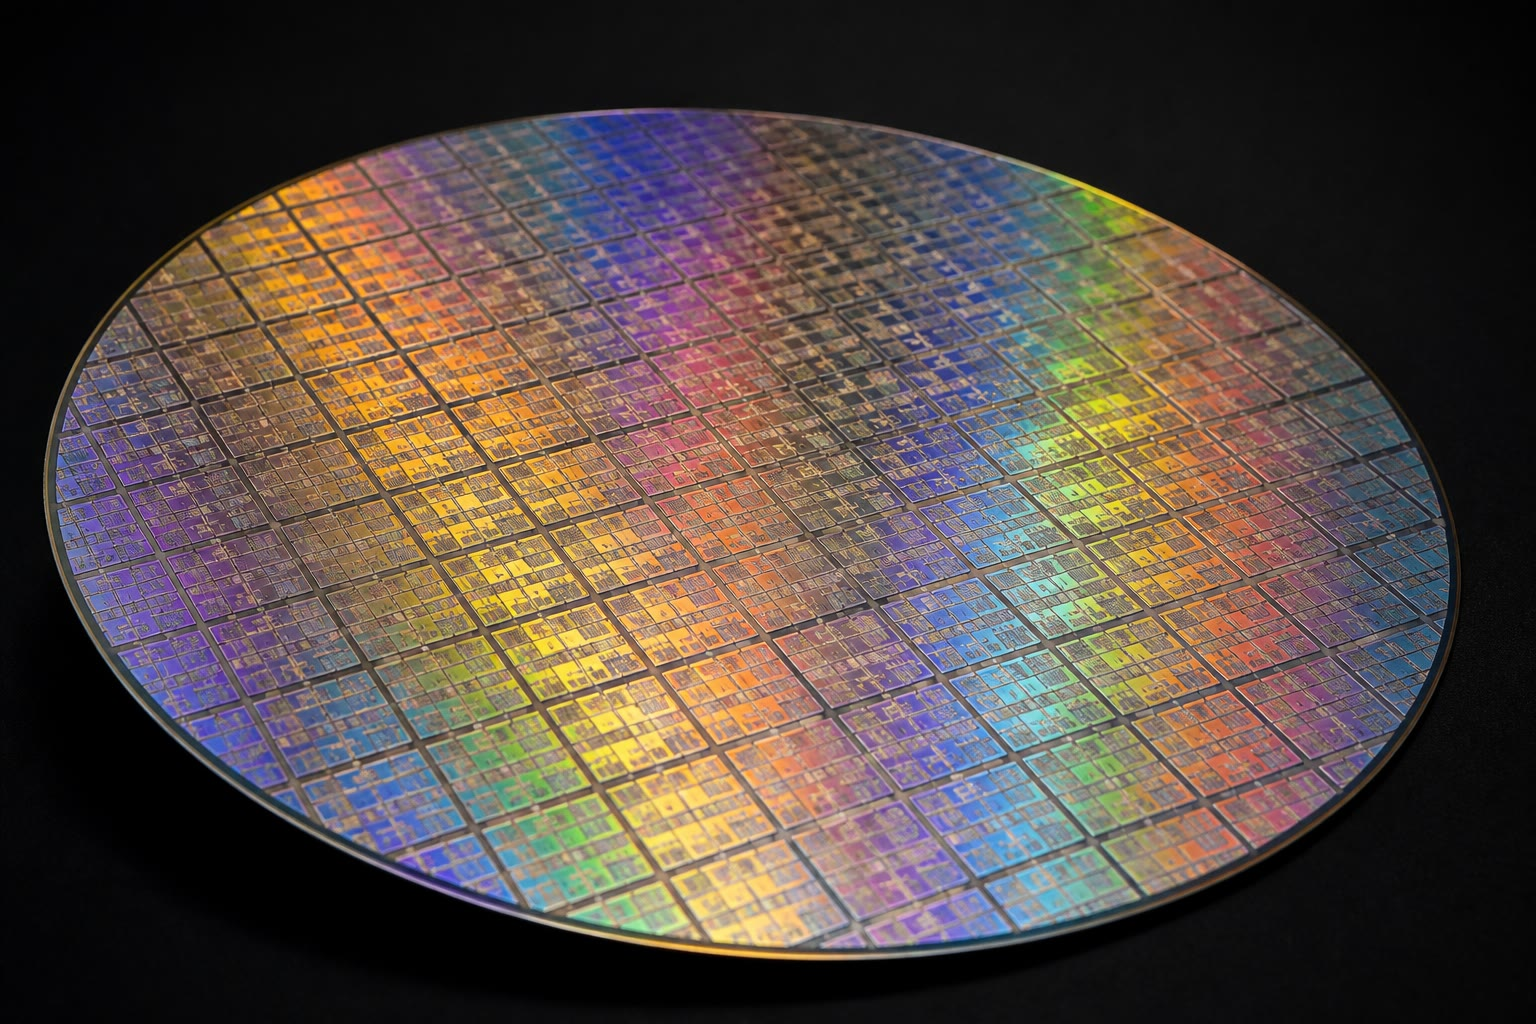
\includegraphics[width=0.58\linewidth]{images/book5/ai/b5-20-silicon-wafer.jpg}

{\small A finished silicon wafer: hundreds of chips, billions of junctions each, printed into one doped \omterm{def:b3:crystalline-solids:lattice}{crystal} --- band theory as the twentieth century's most consequential manufacturing recipe.}
\end{omfigure}

\section{Exercises}

\begin{exercise}[$\star$]\label{exo:b3:electrons-in-solids:1}
Drude's copper. $n = \qty{8.5e28}{m^{-3}}$, resistivity
$\rho = \qty{1.7e-8}{\ohm.m}$. Compute (a) $\tau =
m_{\text{e}}/ne^2\rho$; (b) the mean free path using the Fermi
velocity $v_{\text{F}} = \qty{1.6e6}{m/s}$; (c) that path in
\omterm{def:b3:crystalline-solids:lattice}{lattice constants} ($a = \qty{3.61}{\angstrom}$); (d) explain why
so long a flight already hints that ions themselves do not do the
scattering.
\end{exercise}

\begin{exercise}[$\star$]\label{exo:b3:electrons-in-solids:2}
The snail in the wire. A \qty{1}{mm^2} copper wire carries
\qty{10}{A}. (a) Compute the \omterm{prop:b3:electrons-in-solids:drude}{drift velocity}. (b) How long would
an electron take to cross a \qty{1}{m} lamp cord? (c) Why does
the lamp nevertheless light instantly? (d) Compare
$v_{\text{d}}$ with $v_{\text{F}}$ and comment on Drude's
pinball picture.
\end{exercise}

\begin{exercise}[$\star$]\label{exo:b3:electrons-in-solids:3}
Sorting by bands. Classify, with the band-filling rule: (a)
sodium (one valence electron); (b) magnesium (two --- yet a
\omterm{def:b3:electrons-in-solids:classes}{metal}: what must its bands do?); (c) diamond
($E_{\text{g}} = \qty{5.5}{eV}$); (d) silicon
($\qty{1.12}{eV}$) --- and state for each the sign of
$\dd\rho/\dd T$.
\end{exercise}

\begin{exercise}[$\star$]\label{exo:b3:electrons-in-solids:4}
Gaps and photons. (a) What photon wavelength matches silicon's
gap, and in which spectral region does silicon become
transparent? (b) Same for diamond: why is it clear in the
visible? (c) A gallium nitride LED has $E_{\text{g}} =
\qty{3.4}{eV}$: what colour edge does that set, and why did blue
LEDs need this material? (d) Why does a red LED die dark rather
than glow faintly white when overdriven?
\end{exercise}

\begin{exercise}[$\star\star$]\label{exo:b3:electrons-in-solids:5}
Wiedemann--Franz. (a) From copper's $\kappa =
\qty{400}{W/(m.K)}$ and $\sigma = \qty{5.9e7}{S/m}$ at
\qty{300}{K}, compute $\kappa/\sigma T$. (b) Compare with the
Sommerfeld value $L = \pi^2k_{\text{B}}^2/3e^2 =
\qty{2.44e-8}{W.\ohm/K^2}$. (c) Explain in one sentence why one
kind of carrier ties the two conductivities. (d) Cooking pans
and their handles: use the law to explain a kitchen's material
choices.
\end{exercise}

\begin{exercise}[$\star\star$]\label{exo:b3:electrons-in-solids:6}
The heat-capacity acquittal. (a) Drude predicts
$\tfrac32nk_{\text{B}}$ from the electrons: with copper's $n$,
what fraction would that add to the \omterm{def:b3:crystalline-solids:lattice}{lattice}'s
$3nk_{\text{B}}$ (one conduction electron per atom)? (b)
\Cref{ch:b3:quantum-statistics} instead gives $C_{\text{el}}
\sim \tfrac{\pi^2}{2}nk_{\text{B}}(T/T_{\text{F}})$: evaluate the
suppression $T/T_{\text{F}}$ at \qty{300}{K}
($T_{\text{F}} = \qty{8.1e4}{K}$). (c) Why does the electronic
term nevertheless \emph{win} at liquid-helium temperatures
(recall the \omterm{def:b3:crystalline-solids:lattice}{lattice}'s $T^3$)? (d) What measurement, plotted as
$C/T$ against $T^2$, untangles the two?
\end{exercise}

\begin{exercise}[$\star\star$]\label{exo:b3:electrons-in-solids:7}
The Fermi surface meets the zone. (a) For copper, compute the
Fermi wavelength $\lambda_{\text{F}} = 2\pi/k_{\text{F}}$ with
$k_{\text{F}} = (3\pi^2n)^{1/3}$. (b) Compare with $2a$: how
close is the Fermi surface to the Bragg condition? (c) Explain
physically why the two standing waves at $k = \pi/a$ (charge on
ions versus between them) must differ in energy. (d) Which
experimental fact of \cref{exo:b3:electrons-in-solids:1} does
Bloch's no-scattering theorem finally explain?
\end{exercise}

\begin{exercise}[$\star\star$]\label{exo:b3:electrons-in-solids:8}
The exponential thermometer. Intrinsic silicon has $n_{\text{i}}
\propto \eu^{-E_{\text{g}}/2k_{\text{B}}T}$. (a) Compute the
carrier-density ratio between \qty{400}{K} and \qty{300}{K}. (b)
Hence sketch a thermistor's resistance against temperature and
contrast it with a platinum wire's. (c) Why the factor 2 in the
exponent (what is created \emph{in pairs})? (d) Estimate the
temperature at which silicon electronics fails because intrinsic
carriers swamp a \qty{5e21}{m^{-3}} \omterm{def:b3:electrons-in-solids:doping}{doping}
($n_{\text{i}}(300\,\text{K}) \approx \qty{1e16}{m^{-3}}$).
\end{exercise}

\begin{exercise}[$\star\star$]\label{exo:b3:electrons-in-solids:9}
\omterm{def:b3:electrons-in-solids:doping}{Doping} arithmetic. Silicon has $\qty{5e28}{atoms/m^3}$. (a) One
phosphorus per million silicon atoms: what carrier density, and
what ratio to $n_{\text{i}} \approx \qty{1e16}{m^{-3}}$? (b) By
what factor has one ppm of dirt changed the conductivity? (c)
Explain why \omterm{def:b3:electrons-in-solids:classes}{semiconductor} fabrication first purifies to parts
per \emph{billion} before \omterm{def:b3:electrons-in-solids:doping}{doping} deliberately. (d) Estimate the
average distance between \omterm{def:b3:electrons-in-solids:doping}{donors} and compare with the
\qty{2.4}{nm} orbit of \cref{exo:b3:electrons-in-solids:10}.
\end{exercise}

\begin{exercise}[$\star\star\star$]\label{exo:b3:electrons-in-solids:10}
The \omterm{def:b3:electrons-in-solids:doping}{donor} as a \omterm{thm:b3:hydrogen-atom:levels}{hydrogen atom}. The fifth phosphorus electron
orbits its $+e$ ion \emph{inside} silicon: screen Coulomb by
$\varepsilon_{\text{r}} = 11.7$
(\cref{ch:b3:electromagnetism-in-matter}) and lighten the
electron to its effective band mass $m^* = 0.26\,m_{\text{e}}$.
(a) Scale the hydrogen results of \cref{ch:b3:hydrogen-atom}:
show $E = \qty{13.6}{eV}\times(m^*/m_{\text{e}})/
\varepsilon_{\text{r}}^2$ and evaluate. (b) Compare with
$k_{\text{B}}T$ at \qty{300}{K}: are \omterm{def:b3:electrons-in-solids:doping}{donors} ionised? (c) Scale
the \omterm{thm:b3:hydrogen-atom:levels}{Bohr radius} the same way. (d) The orbit spans dozens of
\omterm{def:b3:crystalline-solids:lattice}{lattice} cells: explain why that self-consistently justifies
using $\varepsilon_{\text{r}}$ and $m^*$ at all.
\end{exercise}

\begin{exercise}[$\star\star\star$]\label{exo:b3:electrons-in-solids:11}
Junction numbers. A silicon diode has $N_{\text{a}} =
N_{\text{d}} = \qty{1e22}{m^{-3}}$, $n_{\text{i}} =
\qty{1e16}{m^{-3}}$, $T = \qty{300}{K}$. (a) Compute
$V_{\text{bi}} = (k_{\text{B}}T/e)\ln(N_{\text{a}}N_{\text{d}}/
n_{\text{i}}^2)$. (b) From the diode law, compute the ratio of
currents at $+\qty{0.5}{V}$ and $-\qty{0.5}{V}$. (c) Why does
$I_0$ --- hence the reverse leak --- roughly double every
\qty{10}{K}? (d) A bridge of four such diodes turns AC into DC:
sketch the circuit's idea in words.
\end{exercise}

\begin{exercise}[$\star\star\star$]\label{exo:b3:electrons-in-solids:12}
Designing the solar gap. (a) Photons below $E_{\text{g}}$ pass
through; photon energy above $E_{\text{g}}$ is lost as heat
within picoseconds. Explain the resulting trade-off in choosing
$E_{\text{g}}$. (b) The optimum near \qty{1.3}{eV} caps
single-junction efficiency at about a third
(Shockley--Queisser): where does silicon
(\qty{1.12}{eV}) stand? (c) Why do tandem stacks (a wide-gap
cell atop a narrow-gap one) beat the cap? (d) Why is a
\emph{hot} solar panel a worse one? (Two chapter-honest reasons:
the diode law's $I_0$, and the gap's slight shrinkage with $T$.)
\end{exercise}

\begin{omfigure}
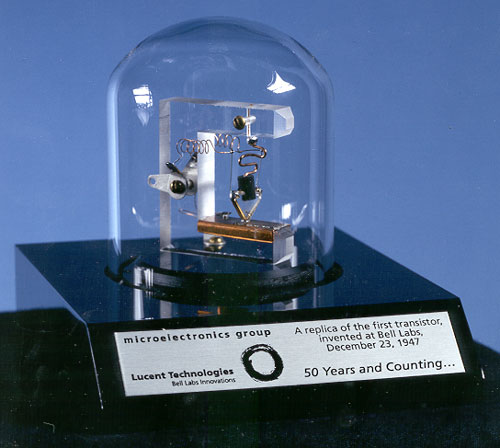
\includegraphics[width=0.45\linewidth]{images/book5/photo-first-transistor.jpg}

{\small Replica of the first transistor (Bell Laboratories, 1947, public domain): two gold contacts pressed onto a sliver of germanium. Band theory's first machine --- and, by descent, all the others.}
\end{omfigure}

\section{Problem: The rooftop referendum}

\begin{problem}\label{pb:b3:electrons-in-solids:1}
\emph{The rooftop referendum.} Your neighbour is deciding whether
to roof their house with photovoltaic panels and has appointed
you, the physicist, as arbiter. The candidate panel: silicon,
\qty{2}{m^2}, sixty cells in series, rated \qty{400}{W} under
the standard \qty{1000}{W/m^2} of noon sunlight.

\medskip\noindent\textbf{Part I --- Sunlight meets the gap.}

\begin{enumerate}
  \item Sunlight is roughly a \qty{5800}{K} thermal spectrum
        (\cref{ch:b3:photons-phonons}): compute the energy of its
        peak photons (Wien) in eV.
  \item Silicon's gap is \qty{1.12}{eV}: what is the longest
        wavelength a silicon cell can harvest?
  \item Roughly a fifth of the sun's power arrives in photons
        below the gap. What happens to it in the panel?
  \item A \qty{2.5}{eV} green photon is absorbed: how much of its
        energy survives as electron--hole pair energy, and where
        does the rest go, and how fast?
  \item Combine items 3 and 4 into the spectrum's verdict: about
        half the incident power is gone before any electronics
        begins. State the two loss channels in one sentence each.
  \item Why does a photon need $\ge E_{\text{g}}$ at all --- what
        forbids absorbing two half-gap photons in quick
        succession in ordinary silicon?
\end{enumerate}

\medskip\noindent\textbf{Part II --- The junction as engine.}

\begin{enumerate}[resume]
  \item Each cell is a \omterm{prop:b3:electrons-in-solids:junction}{p--n junction}. Explain in three sentences
        how the \omterm{prop:b3:electrons-in-solids:junction}{depletion zone}'s built-in field turns a created
        pair into external current --- which carrier goes which
        way, and why they do not simply recombine.
  \item With $N_{\text{a}} = N_{\text{d}} = \qty{1e22}{m^{-3}}$
        and $n_{\text{i}} = \qty{1e16}{m^{-3}}$, compute
        $V_{\text{bi}}$ at \qty{300}{K}.
  \item A working cell delivers about \qty{0.6}{V}. Sixty in
        series: the panel's operating voltage?
  \item From the \qty{400}{W} rating, deduce the operating
        current.
  \item Estimate the photon flux (photons per second) the panel
        absorbs usefully, taking $\sim\qty{2}{eV}$ per absorbed
        photon, and compare with the electron flux your current
        implies: what fraction of absorbed photons yields a
        collected electron?
  \item The rated efficiency: \qty{400}{W} from
        \qty{2000}{W} incident. Reconcile 20\,\% with Part I's
        ``half lost before electronics'': where do the remaining
        thirty points go?
  \item Why does the cell deliver \qty{0.6}{V} and not the full
        \qty{1.12}{V} of the gap? (Name the culprit in the diode
        law.)
\end{enumerate}

\medskip\noindent\textbf{Part III --- Real roofs.}

\begin{enumerate}[resume]
  \item A cloudless winter noon at latitude $50^\circ$ delivers
        light at $30^\circ$ elevation. Compute the geometric
        factor relative to normal incidence on a horizontal
        panel.
  \item The panel datasheet lists $-0.4\,\%/\text{K}$ of output:
        a black roof panel reaches \qty{65}{\celsius} in summer.
        How much of the rating survives?
  \item Explain the temperature loss with
        \cref{exo:b3:electrons-in-solids:12}(d).
  \item A chimney shades one cell of the sixty. Why can that
        strangle the whole series string --- and what does the
        cell's own diode nature do to the poor shaded cell?
  \item Manufacturers wire a \emph{bypass diode} across each
        sub-string: explain its job in one sentence.
  \item Averaged over days and weather, the roof yields
        \qty{15}{\percent} of rated power. Estimate the yearly
        energy from the \qty{400}{W} panel in kilowatt-hours.
\end{enumerate}

\medskip\noindent\textbf{Part IV --- The verdict.}

\begin{enumerate}[resume]
  \item At \qty{0.25}{euros} per kWh, what does the panel earn
        per year? With an installed cost of \qty{300}{euros},
        what is the payback time?
  \item The panel took roughly \qty{500}{kWh} to manufacture
        (silicon is purified by melting): how long until it has
        repaid its own energy?
  \item Your neighbour asks why the panel cannot be
        ``just made black'' to catch the sub-gap fifth. Answer
        with band theory in two sentences.
  \item They ask next why not stack a second, smaller-gap panel
        beneath: answer with
        \cref{exo:b3:electrons-in-solids:12}(c) --- and name the
        practical catch.
  \item Thirty years on, the panel has faded to 85\,\% of its
        rating. Which microscopic villains of this chapter
        (recall what limits $\tau$, and what junctions fear)
        plausibly age a cell?
  \item Deliver the arbiter's summary in four lines: gap physics
        sets the harvest, the junction converts it, series
        wiring and temperature tax it, and the ledger --- energy
        and euros --- closes in the panel's favour.
\end{enumerate}
\end{problem}
